% This is copied from 2017 ESF and it is example of LaTex
% -------------------------------------------------------
% Ondřej Šereda 8.2.2018

\subsubsection{Description/concept}
\iffalse
Describe your concept of the shutdown circuit, the master switches, shut down buttons, brake over travel switch, etc.
Additionally, fill out the following table replacing the values with your specification and append additional switches from your setup:
\fi

Shutdown circuit (SDC) starts in \gls{ecup} unit, then goes through all \gls{sdc} elements in the car and ends in \gls{ecua}, which is placed inside the Accumulator Pack. In \gls{ecup} \gls{sdc} starts from \gls{lv} power +24V and ends in \gls{acp} by powering \gls{air} coils switching circuit (See \ref{fig:SDC-scheme}). The \gls{sdc} consists of 2 master switches, 3 shut-down buttons(SDB), the brake-over-travel-switch(\gls{bots}), the insulation monitoring device (\gls{imd}, the inertia switch, the brake system plausibility device(\gls{bspd}), interlocks in Motor Controllers and Accumulator Pack and the accumulator management system (\gls{ams}) and Front Wheel Interlock(FWIL). FWIL triggers shutdown circuit in case of front suspension failure(see \ref{fig:fwil}). 

\begin{figure}[H]
	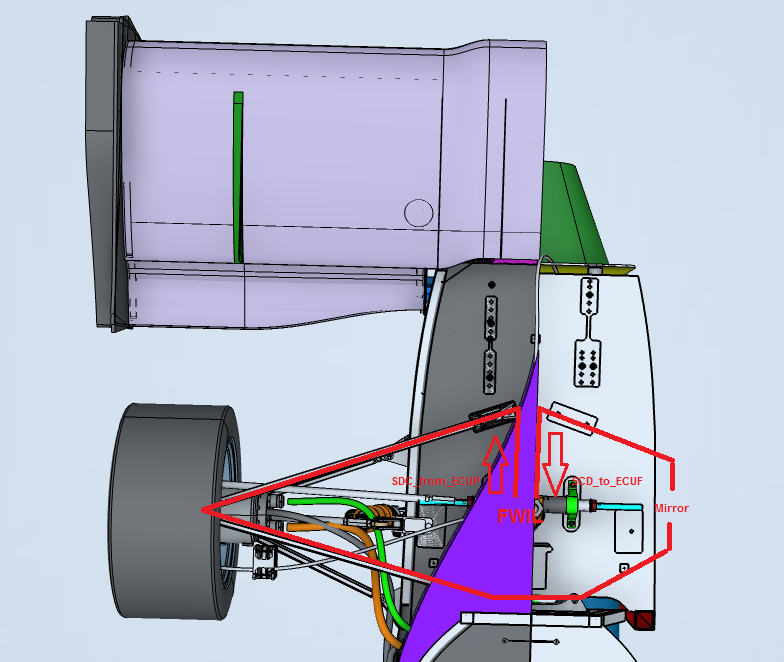
\includegraphics[width=\textwidth]{./img/fwil.png}
	\caption{FWIL positon.}
	\label{fig:fwil}
\end{figure}

All of these crucial parts do not act through any power stage, but carry directly the \gls{air} current.

%\todo[inline]{convert to full name refs}

\begin{figure}[H]
	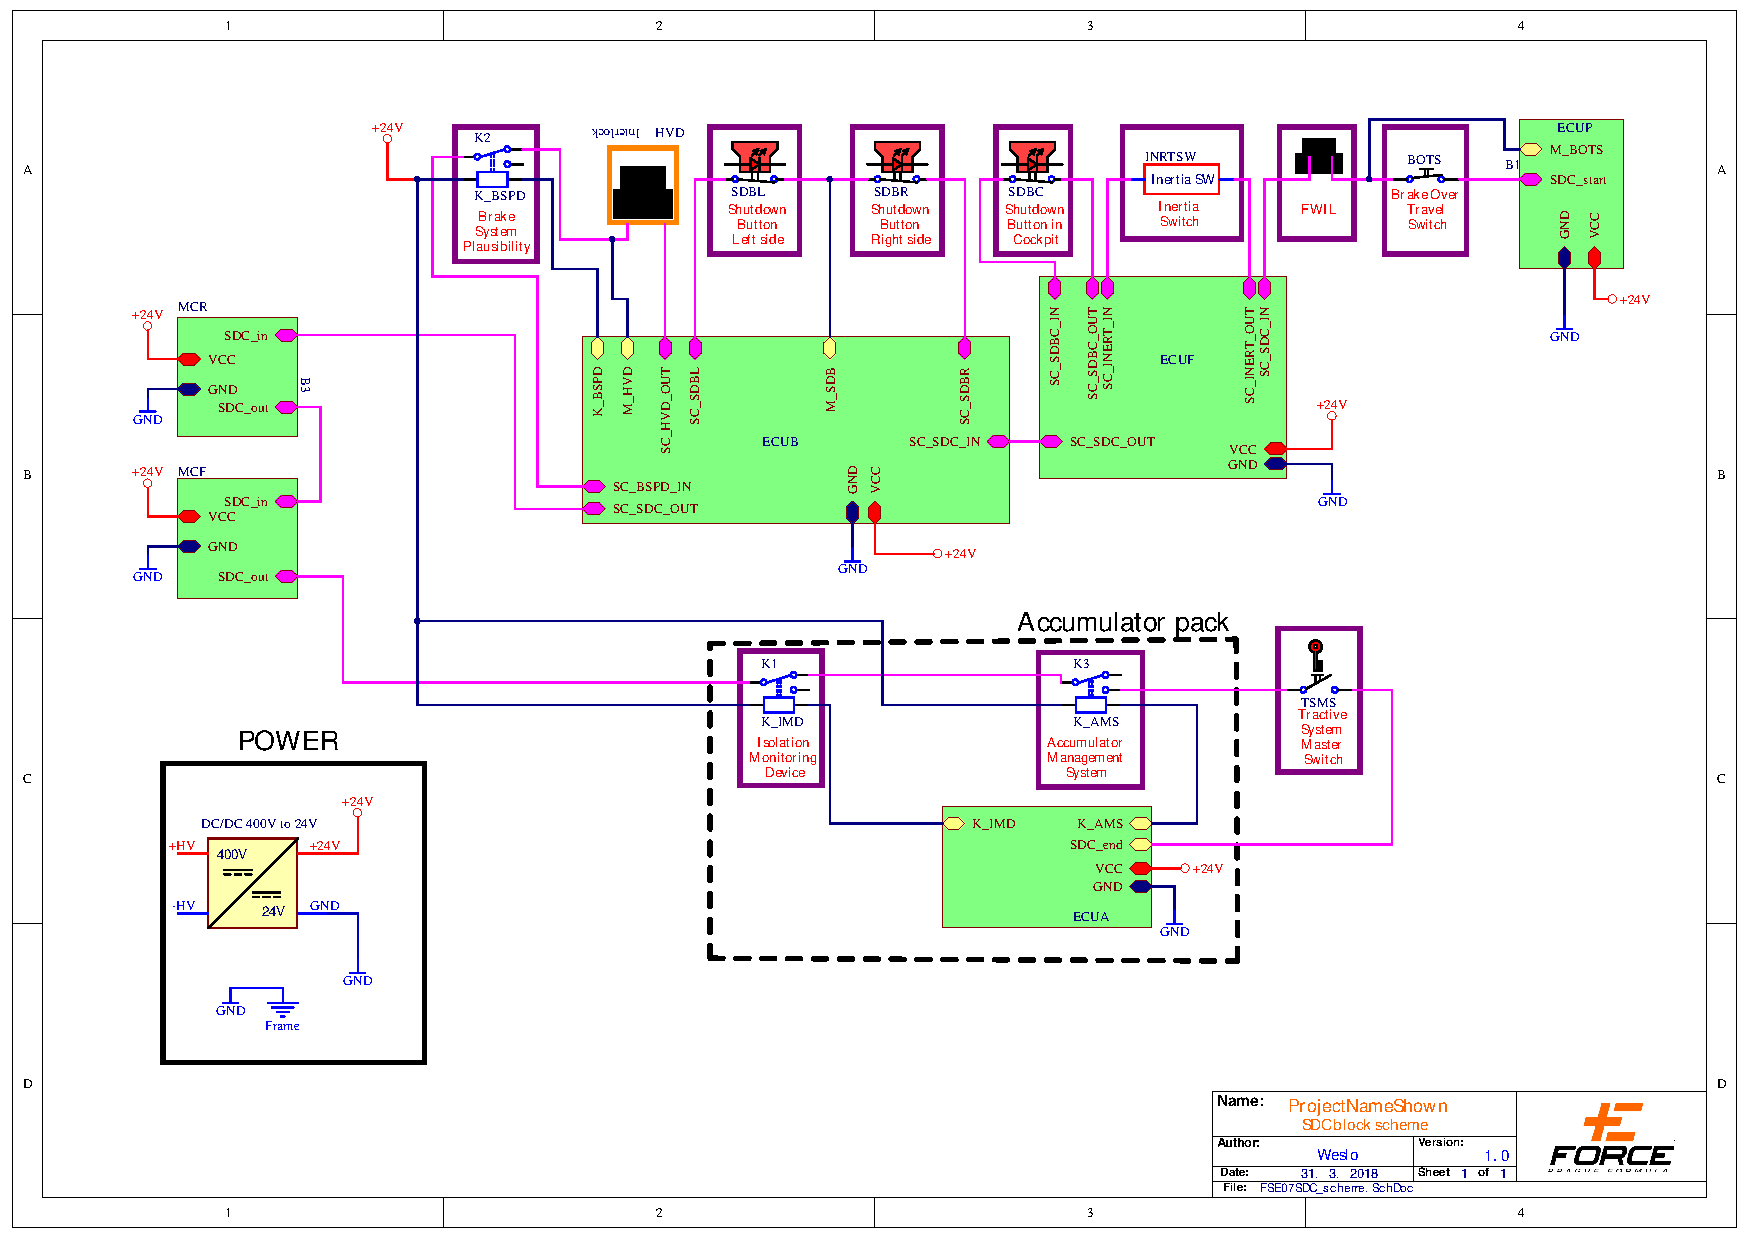
\includegraphics[width=\textwidth, trim={2cm 3cm 2cm 2cm},clip]{./img/SDC-scheme.pdf}
	\caption{\gls{sdc} scheme.}
	\label{fig:SDC-scheme}
\end{figure}

\begin{table}[H]
	\caption{List of switches in the shutdown circuit}
	\centering
	\begin{tabu}{|X|l|}
		\hline Part  & Function \\
		\hline Main Switch (for control and tractive-system; CSMS, TSMS) & Normally open \\
		\hline Brake over travel switch (BOTS) & Normally closed \\
		\hline Shutdown buttons (SDB) & Normally closed \\
		\hline Insulation Monitoring Device (IMD) & Normally open \\
		\hline Battery Management System (BMS) & Normally open \\
		\hline Inertia Switch & Normally closed \\
		\hline Interlocks & Closed when circuits are connected \\
		\hline Brake System Plausibility Device & Normally Open \\
		\hline
	\end{tabu}%
	\label{tab:SDCswitch}%
\end{table}%
\todo[inline]{add refs}

\paragraph{Monitoring SDC}
Every part of \gls{sdc} is monitored by specific \gls{ecu} in order to identify disconnected element. \gls{bots} is measured by \gls{ecup}, SDB-center  and Inertia switch are measured by \gls{ecuf} , interlocks in \glspl{mc} (\gls{fwil}) are measured by \glspl{mc}, Interlock in Accumulator Pack is measured by \gls{ecua}  and finally SDB-right, SDB-left and \gls{tsms} are measured by \gls{ecub}. Every piece of information regarding the state of closure \gls{sdc} are running between ECU´s by \gls{can}. 

We designed \gls{sdc} to be ‘single wire’ alike and distanced it from the system as much as it was possible. In order to remain \gls{sdc} as a stand-alone wire we used optocouplers for main points of \gls{sdc}. Optocouplers are connected in such a way, that they become active only in case of nonzero voltage occurance at a certain point of \gls{sdc}.

\Gls{ecub} is last part of \gls{sdc} before \gls{tsms}. If a state of error on \gls{sdc} is detected \gls{ecub} latches the off-state of \gls{sdc} to stay off. If the occurred error is non-critical, it allows pilot to re-enter the TSON state. If monitored error is critical (such as \gls{imd} etc.), it notes the error to the memory-storage and does not allow \gls{sdc} to become active until appropriate steps are taken.

\paragraph{Master Switch}
We use Autolec Mini-Master battery cut-out switches with continuous current rating 100A, shown on \ref{fig:SDC-TSMS}.
\begin{figure}[H]
	\centering
	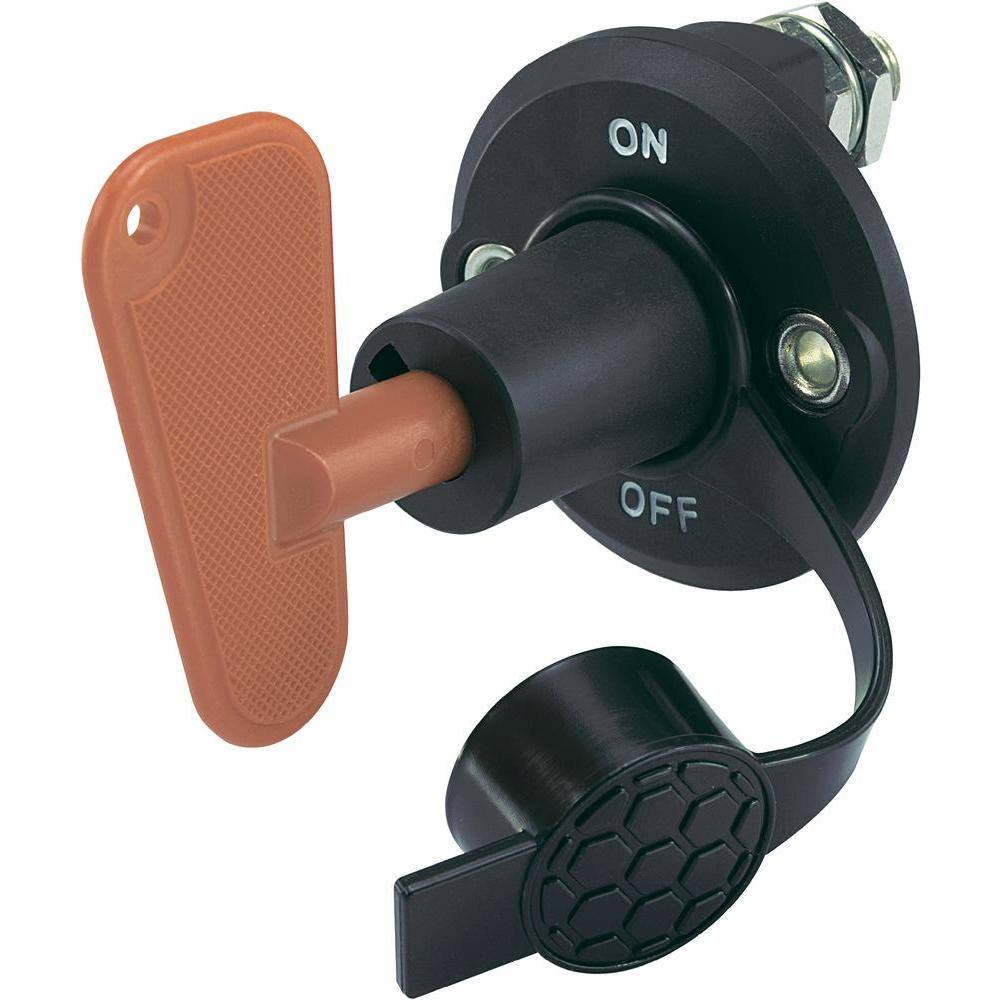
\includegraphics[width=.5\textwidth]{./img/SDC-TSMS.jpg}
	\caption{TSMS.}
	\label{fig:SDC-TSMS}
\end{figure}

\paragraph{Shutdown Switch}
We use OMRON A165E shutdown buttons, which have 3A current rating at 30VDC.

On the cockpit it is OMRON A165E-LS, shown on \ref{fig:SDC-A165E-LS}.
\begin{figure}[H]
	\centering
	\includegraphics[width=.5\textwidth]{./img/SDC-A165E-LS.pdf}
	\caption{Cockpit SDB.}
	\label{fig:SDC-A165E-LS}
\end{figure}

On the left and on the right sides there are OMRON A165E-LM buttons, shown on \ref{fig:SDC-A165E-LM}.
\begin{figure}[H]
	\centering
	\includegraphics[width=.5\textwidth]{./img/SDC-A165E-LM.pdf}
	\caption{SDB left and right.}
	\label{fig:SDC-A165E-LM}
\end{figure}

\paragraph{Brake Over Travel Switch}
It is type A165E-M, current raging 3A, shown on \ref{fig:SDC-A165E-M}
\begin{figure}[H]
	\centering
	\includegraphics[width=.5\textwidth]{./img/SDC-A165E-M.pdf}
	\caption{Brake over travel switch.}
	\label{fig:SDC-A165E-M}
\end{figure}


\subsubsection{Wiring / additional circuitry}
\iffalse
Describe wiring and additional circuitry, show extra schematics for example if additional transistors etc. are used, also describe the function of additional circuitry and make good use of figures.
Additionally, fill out and add information to the following table:
\fi

If connector is used to connect \gls{sdc} between control units, disconnecting any of them results in opening \gls{sdc} and therefore opening \glspl{air} as well. In other words the \gls{sdc} directly carries the current driving the accumulator isolation relays(\glspl{air}). All circuits that are part of the shutdown circuit have been designed in a way, that, when in disconnected state, they remove the current controlling the \glspl{air}.

The cross-section of Shutdown System wire is AWG22. Block wiring scheme shown on \ref{fig:SDC-schematic}.\\

\begin{figure}[H]
	\centering
	\includegraphics[width=\textwidth,trim={4cm 8cm 5cm 3cm}, clip]{./img/SDC-monitoring.pdf}
	\caption{Example of used \gls{sdc} monitoring method with optocouplers.}
	\label{fig:SDC-schematic}
\end{figure}

As shown, 4.7 k$\Omega$ resistors are used to limit current through optocoupler. With 24 V supply that makes 15.2 mA per optocoupler. We used 8 optocouplers: $12*15.2= 182.4$ mA.
% Table generated by Excel2LaTeX from sheet 'List1'
\begin{table}[H]
	\centering
	\caption{Wiring – Shutdown circuit}
	\begin{tabu}{|X|X|}
		\hline
		Total Number of \glspl{air}: & 2 \\
		\hline
		Current per \gls{air}: & 70 mA \\
		\hline
		Additional parts consumption within the shutdown circuit: & 182.4 mA \\
		\hline
		Total current: & 322.4 mA \\
		\hline
		Cross sectional area of the wiring used: & 0.322 mm$^2$ (AWG22) \\
		\hline
	\end{tabu}%
	\label{tab:SDC-Wiring}%
\end{table}%


\subsubsection{Position in car}
\iffalse Provide CAD-renderings showing the relevant parts. Mark the parts in the renderings, if necessary. \fi
\begin{figure}[H]
	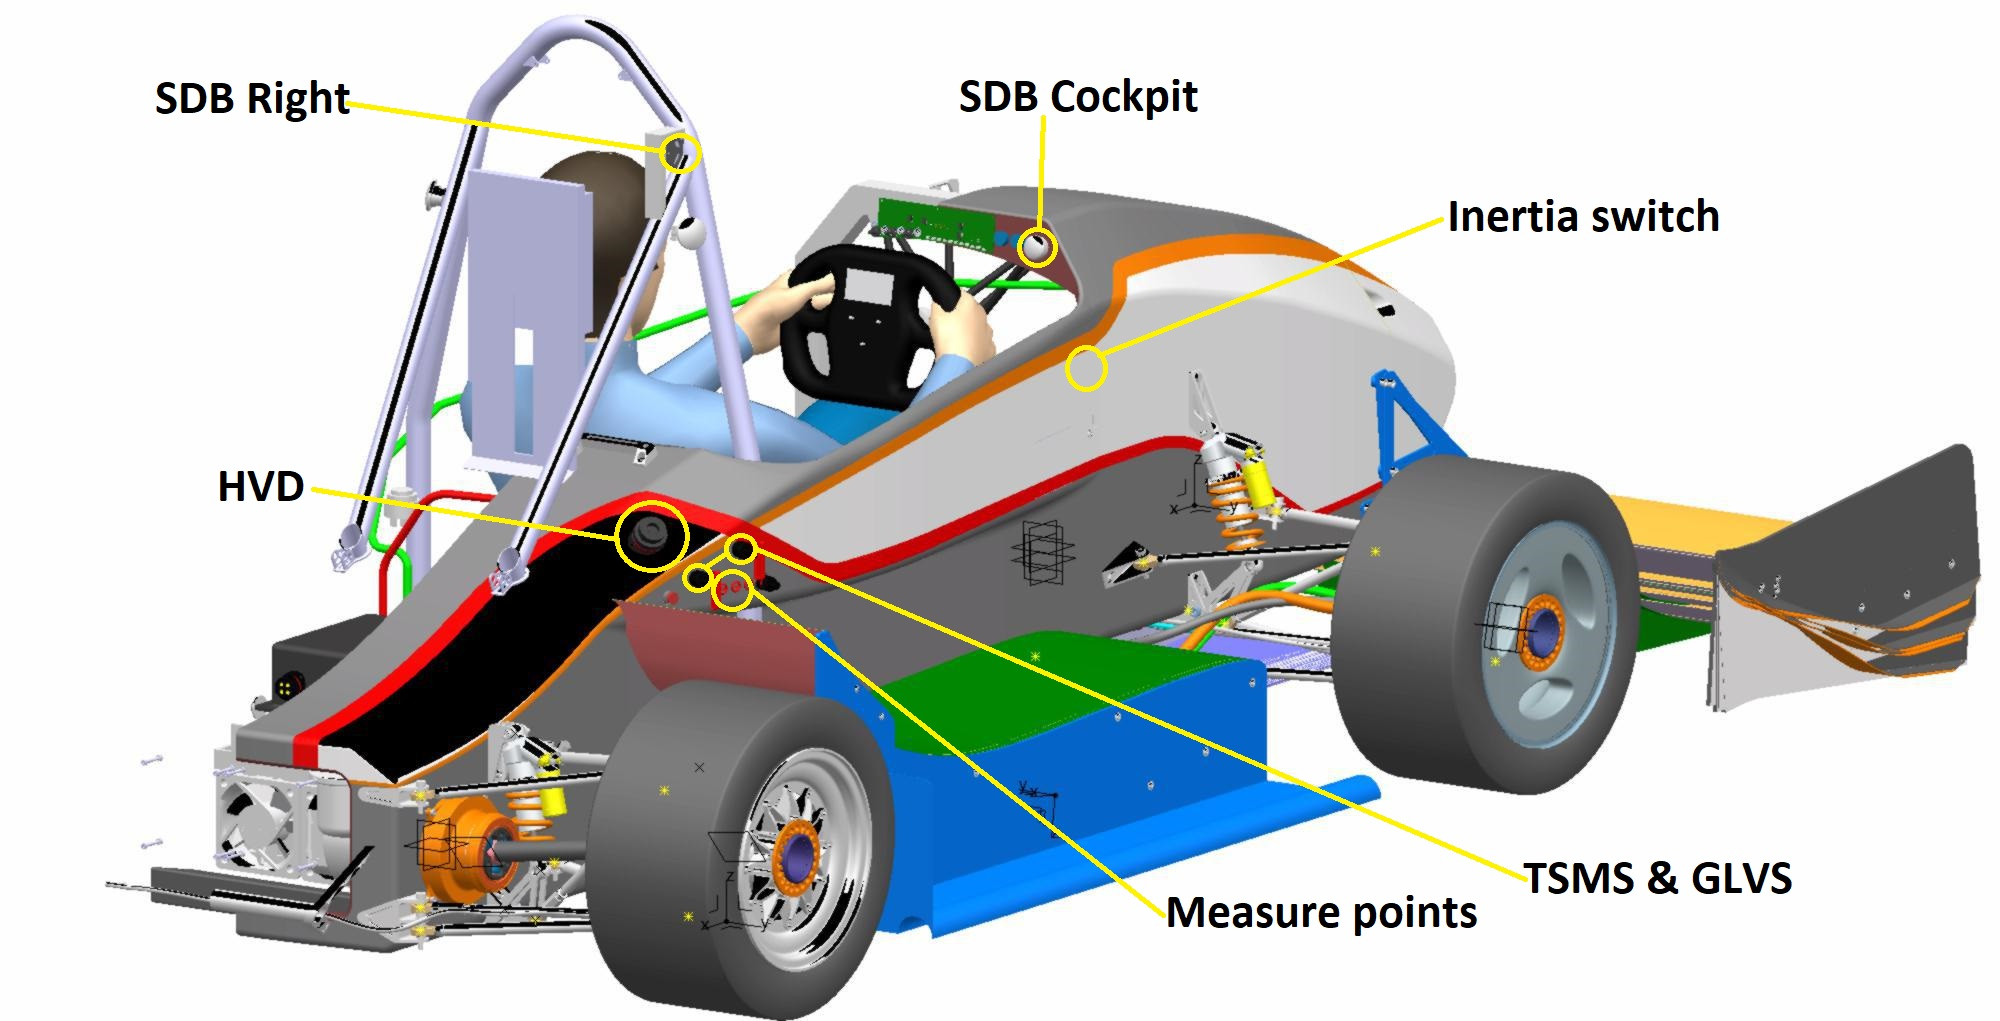
\includegraphics[width=\textwidth]{./img/car-pos.jpg}
	\caption{Inertia switch, SDB Left, Right and Cockpit, \gls{tsms}, \gls{glvms}, HVD, Measure points.}
	\label{fig:SDC-positionInCar}
\end{figure}
